% -*- mode: LaTeX; mode: TeX-PDF; coding: utf-8  -*-

\documentclass[pdf, 9pt, unicode]{beamer} %Для tex -> pdf
%unicode - обязательно (почему не ясно)
%9pt надо подобрать

%Пакеты для русского языка

\usepackage[cp1251]{inputenc}
\usepackage[russian]{babel}
\usepackage[T2A]{fontenc}


\usepackage{amsfonts}
\usepackage{amssymb}
\usepackage{amsthm}
\usepackage{amsmath}

\usepackage{indentfirst}
\usepackage{newlfont}
\usepackage{mathtext}        % еcли нyжны pyccкие бyквы в фоpмyлах

\usepackage{bm,times}

\usepackage{verbatim}

%\usecolortheme{default}
% путь к рисункам
\graphicspath{{images/}}

%Привычный шрифт для математических формул
\usefonttheme[onlymath]{serif}

%Задание команды (\bluetext) для выделения конкретным (синим) цветом
%(используйте \alert для выделения цветом выбранной "темы")
\setbeamercolor{bluetext_color}{fg=blue}
\newcommand{\bluetext}[1]{{\usebeamercolor[fg]{bluetext_color}#1}}

%Если используется последовательное появление пунктов списков на слайде
%(не злоупотребляйте в слайдах для защиты дипломной работы), чтобы
%еще непоявившиеся пункты были все-таки немножко видны.
%\setbeamercovered{transparent}


%Общий стиль ("тема") оформления слайдов
%Можно выбрать любую тему в \localtexmf\tex\latex\beamer\themes\theme\
%и ее имя подставить в качестве аргумента в \usetheme

%\usetheme {Frankfurt}
%\usetheme {Madrid}
%\usetheme {Warsaw}
%\usetheme {Rochester}
%\usetheme {Marburg}

%\useoutertheme {shadow}

% тоже  задается стиль 
\usepackage{beamerthemesplit} 

%Более крупный шрифт для подзаголовков титульного листа                                                                      
\setbeamerfont{institute}{size=\normalsize}

\setbeamercolor{bluetext_color}{fg=blue}
\renewcommand{\alert}[1]{{\usebeamercolor[fg]{bluetext_color}#1}}


\setbeamercolor{block title}{fg=white, bg=blue}
%\setbeamerfont{block title}{family = \sffsmily}
\setbeamercolor{block body} {bg = white}
\setbeamertemplate{blocks}[rounded][shadow = true]


\title[
%Алгоритмы сглаживания на базе обобщенных средних В. А. Стеклова
Алгоритмы сглаживания при восстановлении функций
]
{
АЛГОРИТМЫ СГЛАЖИВАНИЯ  
НА БАЗЕ ОБОБЩЕННЫХ СРЕДНИХ В.~А.~СТЕКЛОВА 
ПРИ ВОССТАНОВЛЕНИИ ФУНКЦИЙ ПО ИЗВЕСТНЫМ
ЗНАЧЕНИЯМ В УЗЛАХ
} 
\date{
%ОАО <<Концерн <<Океанприбор>>\\
%СПб НИУ ИТМО\\
Санкт-Петербург\\2013
}

\author[
Елена Сергеева
]{
Елена Сергеева\\ 
%\bigskip
%Елена Сергеева
%\and ОАО <<Концерн <<Океанприбор>>
}

\institute{
%ОАО <<Концерн <<Океанприбор>>
научный руководитель:\\ к.ф.-м.н. Г. Ю. Пуеров\\
\bigskip
СПб НИУ ИТМО
}

\begin{document}


\begin {frame}
  \titlepage
\end{frame}

\begin{frame}
  \frametitle{Постановка задачи}

\label{net}
\centering
\begin{minipage}[h]{0.75\linewidth}
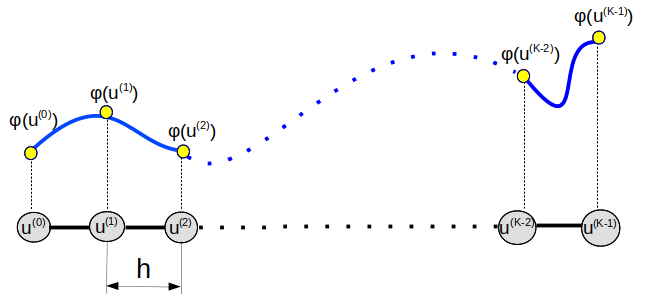
\includegraphics[
width = 1\linewidth
]{net}
\end{minipage}
\begin{block}{Требуется}
Найти гладкую, достаточно <<простую>> функцию %$g$
<<хорошо>> аппроксимирующую исходную функцию $\varphi$.
\end{block}
\end{frame}


\begin{frame}
  \frametitle{Определения: Средние В. А. Стеклова}

\begin{block} {Для функции одной переменной} 
    %\alert{Для функции одной переменной} 

    Пусть $f$ --- локально суммируемая функция, $w>0,\ r-1 \in \mathbb{N}.$
    \begin{align*}
      &S_{w,1}(f)=\frac{1}{w}\int\limits_{-w/2}^{w/2} f(\cdot+t)\,dt,\\
      &S_{w,r}(f)=S_{w,1}(S_{w,r-1}(f)).
    \end{align*}
    % Функция $S_{w,r}(f)$ называется средним В.~А.~Стеклова  порядка $r$ с шагом
    % $w$ функции~$f.$  
\end{block}

\begin{block}{В двумерном случае} 
   % \alert{В двумерном случае} 

    Если рассматривается некоторая величина $x\in\mathbb{R}^2,$ то
    $x_k$ ($k=1,2$) обозначает ее $k$-ю координату.
 
    Пусть $r=(r_1,r_2),\ r_1, r_2 \in \mathbb{N},\ w = (w_1,w_2),\ w_1,w_2 > 0.$ 
    \begin{equation*}
      S_{w,r}(f)=S_{w_1,r_1}S_{w_2,r_2}(f).
    \end{equation*}
\end{block}
\end{frame}


\begin{frame}
  \frametitle{Определения: Ядра В. А. Стеклова}

\begin{block}{В одномерном случае}
  %  \alert{В одномерном случае}

    Пусть $ r\in \mathbb{N},\ t\in\mathbb{R},\ w>0.$ 
    \begin{align*}
      \psi_r(t)&=
      \begin{cases}
        \frac{1}{(r-1)!}\sum\limits_{0\leqslant k<\left(|t|+\frac{r}{2}\right)}(-1)^kC_r^k\left(|t|+\frac{r}{2}-k\right)^{r-1},&\ \text{если}\ |t|\leqslant r/2,\\
        0,&\ \text{если}\ |t| > r/2,
      \end{cases} \\
      \psi_{w,r}(t)&=\frac{1}{w}\psi_r\left(\frac{t}{w}\right).
    \end{align*}
\end{block}

\begin{block}{В двумерном случае}
%    \alert{В двумерном случае}

    Если рассматривается некоторая величина $x\in\mathbb{R}^2,$ то
    $x_k$ ($k=1,2$) обозначает ее $k$-ю координату.
 
    Пусть $t=(t_1,t_2),\ r=(r_1,r_2),\ r_1,r_2 \in \mathbb{N},\  w = (w_1,w_2),\ w_1,w_2 > 0.$
    \begin{equation*}
      \psi_{w,r}(t)=\psi_{w_1,r_1}(t_1)\psi_{w_2,r_2}(t_2).
    \end{equation*}
\end{block}

\end{frame}


\begin{frame}
\frametitle{Определения}

\begin{block} {Пример ядер В. А. Стеклова}
%\alert{Пример ядер Стеклова для}
     \begin{align*}
        &\psi_{2}(t)=
        \begin{cases}
          1-|t|,
          &\ \text{если}\ |t|\leqslant 1,\\
          0,&\ \text{если}\ |t| > 1.
        \end{cases}
        \\
        &\psi_{4}(t)=\frac{1}{6}
        \begin{cases}
          3|t|^3-6t^2+4,
          &\ \text{если}\ |t|\leqslant 1,\\
          -|t|^3+6t^2-12|t|+8,
          &\ \text{если}\ 1<|t|\leqslant 2,\\
          0,&\ \text{если}\ |t| > 2.
        \end{cases}
      \end{align*}
\end{block}


\begin{block}{Связь средних и ядер В. А. Стеклова}
%\alert{Связь средних и ядер Стеклова}
%Пусть $w>0,\ p-1 \in \mathbb{N}, .$
$$
S_{w,r}(f,x)=\int\limits_{\mathbb R} f(x+t)\psi_{h,r}(t)\,dt.
$$
Отметим, что
$$
S_{w,r}(\psi_{w,p},t) = \psi_{w,r+p}(t).
$$
\end{block}

\end{frame}


\begin{frame}
\frametitle{История вопроса}
%В работе \cite{Zhuk} предложен следующий подход 
\Large{
\begin{itemize}
\item 
В.~В.~Жук (1993)  предложил следующий подход к решению поставленной задачи:


\begin {enumerate}
\large{
\item 
Строится непрерывная функция, интерполирующая исходные данные, %в узлах равномерной сетки, 
%причем 
значения в узлах $u^{(\boldsymbol{l})}$ берутся с весом $h_1h_2\psi_{h,(2,2)}(\cdot-u^{(l)}).$
}
\item 
\large{
С помощью средних В.~А.~Стеклова $S_{\boldsymbol{h},\boldsymbol{r}}$ производится сглаживание.
%Важнейшим обстоятельством данного подхода является то, что все операции удается осуществить в конечной
%форме, не прибегая к приближенным методам.
}
\end{enumerate}

\item
Н.~И.~Ахиезер (1947) 
рассмотрел оператор $I_{n,r} = E - (E-I_n)^r$,\\ где $E$ --- тождественный оператор, $I_n$ --- интеграл Валле-Пуссена.

%\item 
%Предлагается для сглаживания
%использовать следующее обобщение средних В.~А.~Стеклова % \cite{DronZhuk,Puerov}
%%(определение в моей статье --- во вложении)
% \begin{equation*}
%     S_{\boldsymbol{h},\boldsymbol{r},m}(f)=(E-(E-S_{\boldsymbol{h},\boldsymbol{r}})^m)(f),
% \end{equation*}
%где $E$ --- тождественный оператор, $m \in \mathbb{N}$. 

%\item 
%Использование обобщенных средних В.~А.~Стеклова позволит 
%получить более высокую точность аппроксимации при сохранении вычислительной 
%эффективности.

\end{itemize}
}
\end{frame}

\begin{frame}
  \frametitle{Алгоритм построения аппроксимирующей функции}
  \begin{enumerate}
  \item 
%Этап 1
%Строится непрерывная функция, интерполирующая исходные данные в узлах равномерной сетки:
%Строится суммарный оператор
% \begin{equation*}
%   G_h(\varphi,x) = h_1 h_2 \sum {\varphi(u^{(l)})\psi_{h,(2,2)}(x-u^{(l)})}
% \end{equation*}
% %если $x$ лежит в определенной ячейке, то суммирование распостраняется на ее вершины


Строится аппроксимирующий оператор следующим образом
% \begin{equation*}
%   G_{h,m}(\varphi,x) = (E-(E-G_h)^m)(\varphi,x),  
% \end{equation*}
%где
 \begin{equation*}
   G_h(\varphi,x) = h_1 h_2 \sum {\varphi(u^{(l)})\psi_{h,(2,2)}(x-u^{(l)})}.
 \end{equation*}


  \item 
%Этап 2
К построенному на шаге 1 оператору применяется сглаживание:
 \begin{equation*}
     S_{h,r,m}(G_{h}(\varphi))=(E-(E-S_{h,r})^m)(G_{h} (\varphi)),
 \end{equation*}
где $E$ --- тождественный оператор, $m \in \mathbb{N}$. 
\end{enumerate}

\begin{block}{Примечание}
Так как
$
S_{h,p}(\psi_{h,r},t) = \psi_{h,r+p}(t),
$
то сглаженная функция является комбинацией ядер В.~А.~Стеклова.
\end{block}
\end{frame}


\begin{frame}
  \frametitle{Пример}

%Например, если $m=2,\ r=(2,2),$ то
%$$
%S_{h,(2,2),2}(g,x) = h_1 h_2 \sum_k \varphi(u^{(k)})\left(2 \psi_{h,(4,4)}(x-u^{(k)}) - \psi_{h,(6,6)}(x-u^{(k)})\right).
%$$ 

\begin{block}{При $m=2, r=(2,2)$}
$$
S_{h,(2,2),2}(G_{h}(\varphi)) = h_1 h_2 \sum_l \varphi(u^{(l)})\left(2 \psi_{h,(4,4)}(x-u^{(l)}) - \psi_{h,(6,6)}(x-u^{(l)})\right)
$$ 

%  \begin{align*}
%    S_{h,r,2}(G_{h,2}) = h_1 h_2 \sum_l \varphi(u^{(l)})\left(&2 \psi_{h,(r_1+2,r_2+2)}(x-u^{(l)}) - \%\ 
%      &- \psi_{h,(2r_1+2,2r_2+2)}(x-u^{(l)})\right).
%  \end{align*}
\end{block}


\label{ext_net}
\centering
\begin{minipage}[h]{0.6\linewidth}
\includegraphics[
width = 1\linewidth
]{ext_net}
\end{minipage}

 % $x \in [lh,(l+\mathbf{1}^2)h]$, 
 % $l \in [\mathbb{O}^2, p-\mathbf{1}^2] \cap \mathbb{Z}^2$

%Сетка должна быть расшеренная --- объяснить.

\end{frame}


\begin{frame}
  \frametitle{Оценка ошибки сглаживания}

Пусть 
\begin{itemize}

\item
$h_1, h_2 > 0$,
$r_1, r_2 \in \mathbb{N}$, 
$m \in \mathbb{N}$;
%$1\leqslant p \leqslant \infty$;

\item
$f$ --- $2m$-гладкая на выпуклой области $G\subset\mathbb{R}^2$ функция; 

\item
прямоугольник $[-\frac{mh_1r_1}{2},a_1+\frac{mh_1r_1}{2}]\times[-\frac{mh_2r_2}{2},a_2+\frac{mh_2r_2}{2}] \subset G$;

\item
$\|f\|_{Q,\infty}=\sup\limits_{x\in Q}|f(x)|;$

%\item
$  \|f\|_{Q,p}=\left(\int\limits_{Q}|f|^p\right)^{1/p},$
если $f$ измерима на $Q,\ 1\leqslant p < \infty$; 

\item
$
\mathcal{D}_{2m}f(x) =  \sqrt{\sum\limits_{k=0}^{2m}C_{2m}^{k}\left (\frac{\partial^{2m} f(x)}{\partial x_1^{k} \partial x_2^{2m-k}}\right)^2}.
$

\end{itemize}

\begin{block}{Оценка} 
  \begin{equation*}
\|f-S_{h,r,m}(f)\|_{[0,a_1]\times[0,a_2],p}\leqslant \left(\frac{(r,h^2)}{24}\right)^m\Lambda_{\frac{mhr}{2},m}(f)_p,
  \end{equation*}
%}
%}
где
$  
\Lambda_{\frac{mhr}{2},m}(f)_p=\|\mathcal{D}_{2m}f\|_{[-\frac{mh_1r_1}{2}, a_1+\frac{mh_1r_1}{2}]\times[-\frac{mh_2r_2}{2},a_2+\frac{mh_2r_2}{2}],p}.
$
\end{block}
\end{frame}


\begin{comment}
\begin{frame}
    \frametitle{Оценка ошибки сглаживания}

\begin{block}{Оценка} 
%Тогда выполнена оценка
\Large{
\alert{
  \begin{equation*}
    \|S_{h,(2,2),m}(f)-f\|_{[0,a_1]\times[0,a_2],p}\leqslant \left(\frac{1}{12}\right)^m|h|^{2m}\Lambda_{h,m}(f)_p,    
  \end{equation*}
}
}

где,

$$  \Lambda_{h,m}(f
)_p=\|\mathcal{D}_{2m}f\|_{[-mh_1,a_1+mh_1]\times[-mh_2,a_2+mh_2],p}.
$$


% \begin{itemize}
% \item
% %\begin{equation*}
% $  \Lambda_{h,m}(f
% %,[0,a_1]x[0,a_2]
% )_{\infty}=\sup_{\tau\in[-mh_1,a_1+mh_1]\times[-mh_2,a_2+mh_2]}\mathcal{D}_{2m}f(\tau)$,
% %\end{equation*}

% %если $p = \infty$
% \item
% %\begin{equation*}
% $  \Lambda_{h,m}(f
% %,[0,a_1]x[0,a_2]
% )_p=\sup_{\tau\in[-mh_1,mh_1]\times[-mh_2,mh_2]}\|\mathcal{D}_{2m}f\|_{[-\tau_1, a_1+\tau_1]\times[-\tau_2, a_2+\tau_2],p}$.
% %\end{equation*}

% %если $1\leqslant p < \infty$.
% \end{itemize}


\end{block}

\end{frame}
\end{comment}

\end{document}







